%%%%%%%%%%%%%%%%%%%%%%%%%%%%%%%%%%%%%%%%%%%%%%%%%%%%%%%%%%%%%%%%%%%%%%%%%%%%%%%%%%%%%%%%%%%%%
%%									Chapitre 3												%
%%%%%%%%%%%%%%%%%%%%%%%%%%%%%%%%%%%%%%%%%%%%%%%%%%%%%%%%%%%%%%%%%%%%%%%%%%%%%%%%%%%%%%%%%%%%%

\chapter{Vision événementielle et attention}
	\citationChap{
		On ne voit que ce que l'on regarde.
	}{Maurice Merleau-Ponty}
	\minitoc
	\newpage

%%%%%%%%%%%%%%%%%%%%%%%%%%%%%%%%%%%%%%%%%%%%%%%%%%%%%%%%%%%%%%%%%%%%%%%%%%%%%%%%%%%%%%%%%%%%%



% Début du chapitre			
	\section{Introduction}
	\section{Détection de mouvements}

	Le rôle de la première couche pour traiter les événements de la caméra sera de transformer les informations ponctuelles dans le temps et l'espace qu'envoie la caméra en zones de mouvements continues, facilitant le travail des couches supérieures. Pour ce faire, nous utiliserons des DNF, particulièrement appropriés par leur capacité d'intégration de l'information, et de leur robustesse au bruit très présent dans ce type de caméra. Habituellement, on utilise des DNF à deux dimensions pour gérer des images. Cependant cela représente 307 200 neurones avec notre caméra 640$\times$480, tous connectés dépendants les uns des autres, et devant être recalculés à chaque itération. Nous souhaitons que la première couche soit simple et rapide, alors nous avons choisi d'utiliser deux DNF à une dimension, un pour chaque axe.

	\begin{figureth}
		\begin{subfigureth}{\textwidth}
			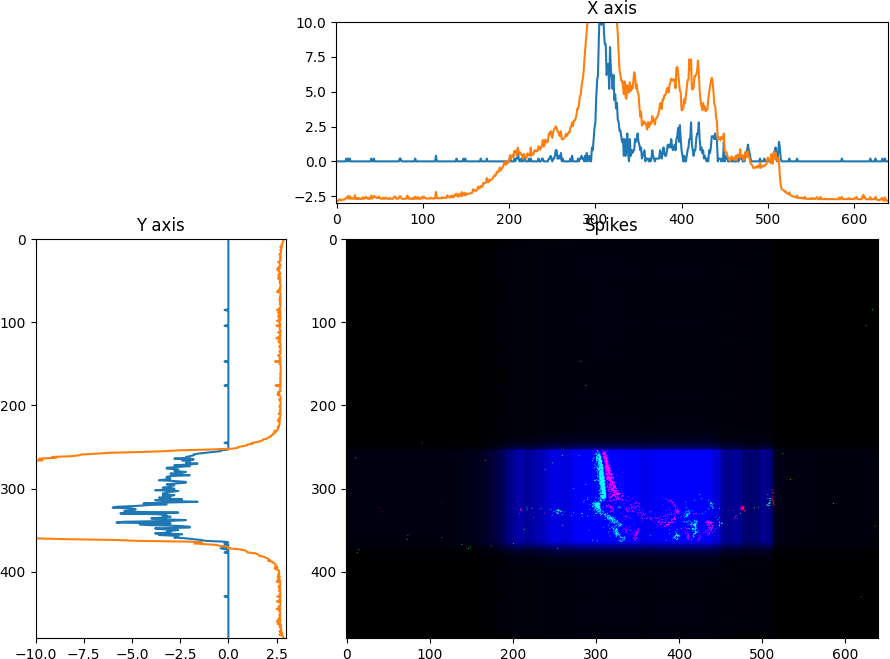
\includegraphics[width=\linewidth]{tracking/plane}
		\end{subfigureth}
		\caption[Détection de mouvements avec DNF sur caméra événementielle]{Détection de mouvements avec DNF sur caméra événementielle. Les points verts et rouges dans l'image correspondent respectivement aux augmentations et réductions de luminosités détectés par la caméra. La somme des événements de chaque axe est affichée dans les courbes bleues qui sont en entrée des deux DNF. En orange sont les potentiels des DNF. On calcule le produit dyadique de la sortie des DNF, c'est à dire après la sigmoïde, pour obtenir la zone de détection de mouvement en bleu sur l'image.}\label{fig:track:plane}
	\end{figureth}

	Les DNF peuvent fonctionner à la fois en mode impulsionnel et en mode discrétisé. Nous avons choisi le second mode, car il est plus rapide à calculer et plus stable. Sa vitesse ne dépend pas du nombre d'événements à traiter, contrairement au modèle impulsionnel. Il nous a donc fallu intégrer les évènements avec un pas de temps que nous avons mis à 10 ms. Il est aussi possible de le placer à 1 ms ou en dessous, si l'on souhaite détecter des mouvements très rapides. Il y aura juste plus de mises à jour par seconde des potentiels du DNF, et donc plus de calculs. Nous n'avons pas utilisé la polarité des évènements, uniquement si un pixel détectait un changement ou pas.

	Les événements que nous recevons de la caméras sont très bruités. Il existe notamment certains pixels défectueux qui envoient en permanence des événements. Il s'agit de bruit artificiel dû à la technologie et non présent dans la nature. Il n'est donc pas particulièrement intéressant pour nous de l'inclure dans notre étude. Nous avons donc désactivé logiciellement ces pixels défectueux. Le bruit présent dans la nature et plus diffus, a lui été conservé. Le résultat est présenté sur la figure \ref{fig:track:plane}.

	\subsection{Multi cibles}

	\begin{figureth}
		\begin{subfigureth}{\textwidth}
			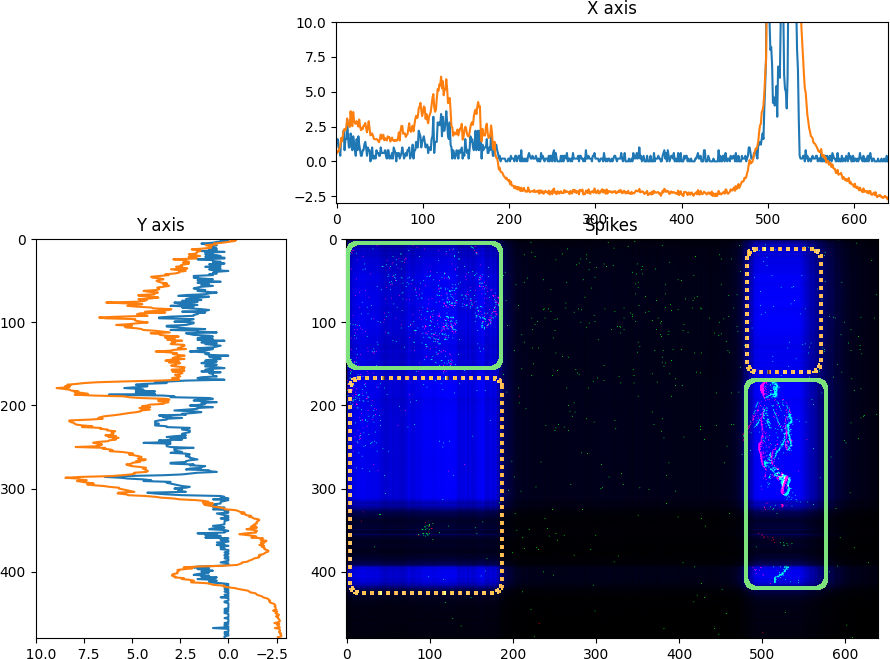
\includegraphics[width=\linewidth]{tracking/walk_with_contours}
		\end{subfigureth}
		\caption[Détection de mouvements multicible avec DNF sur caméra événementielle]{Détection multicible. Il y a deux stimulus dans la scène, entourés par des lignes vertes. La personne qui se déplace en bas à droite et un mouvement dans un arbre en haut à gauche. Les activations parasites, dû à la projection de deux détections en 1D vers du 2D sont entourés par des pointillés orange.}\label{fig:track:multi}
	\end{figureth}

	Notre système est également capable de suivre de multiples cibles, mais au prix de détections parasites. En effet, passer de 2 dimensions à 2 fois 1 dimension pour ensuite projeter à nouveau en 2 dimensions est efficace en calculs, mais il y a une perte d'informations dans le processus. Lorsque l'on passe en 1 dimensions, on ne connaît que les valeurs sur chaque axe des deux stimulus, sans pouvoir les associer entre elles. Un exemple est présenté sur la figure \ref{fig:track:multi}.

	\subsection{Paramètres}

	Le paramétrage de DNF est une tâche délicate. Nous avons ajusté à la main les valeurs de chaque paramètre à l'aide de nos connaissances sur ces modèles. Bien que nous n'ayons pas beaucoup modifiés les paramètres entre les deux exemples que nous avons présentés, il est possible qu'une séquence nouvelle ne fonctionne pas avec les paramètres que nous avons sélectionnés, et qu'il faille reparamétrer les DNF pour que cela fonctionne comme attendu. Les deux DNF de chaque axe utilisent les mêmes paramètres. Chaque événement compte pour 0.2 dans l'entrée des DNF pour une meilleure visualisation sur les figures, car mettre cette valeur à 1 et diviser le gain par 5 aurait eu le même effet sur le DNF.


	\begin{tableth}
	\label{tab:recap:param}
	\caption[Paramètres DNF 1D]{Paramètres DNF 1D}
	\begin{tabular}{|c|cc|}
		\hline
		Paramètre & Figure \ref{fig:track:plane} & Figure \ref{fig:track:multi}\\
		\hline
		$\delta$t & 0.01 & 0.01\\
		$\tau$ & 0.05 & 0.05\\
		Coef. excitateur & 4.5 & 4.5\\
		$\sigma$ excitateur & 0.01 & 0.01\\
		Gain & 4 & 1.5\\
		Repos $h$ & -3 & -3\\
		\hline
	\end{tabular}
	\end{tableth}

	\newpage

	\section{Combinaison avec la détection de nouveauté}

	La détection de mouvement présentée dans la section précédente a des points communs avec la détection de nouveauté de la SOM. En effet, chaque cible détectée par la détection de nouveauté sera nécessairement également détectée par la détection de mouvement. Car la nouveauté ne peut apparaître qu'avec du mouvement. L'inverse n'est cependant pas vrai (il peut y avoir du mouvement sans nouveauté), et ce principe ne compte que lors de l'apparition de nouveauté. Si de la nouveauté s'arrête de se déplacer, elle n'apparaîtra plus comme mouvement, mais sera toujours de la nouveauté.

	La détection de mouvement étant beaucoup plus rapide que la détection de nouveauté, nous pouvons utiliser celle-ci comme déclencheur de la détection de nouveauté dans une zone particulière de l'image. Ainsi, la détection de nouveauté ne sera appelée que lorsque du mouvement apparaîtra dans l'image, et limitera le calcul de la SOM à une zone d'intérêt dans l'image. Un exemple est montré sur la figure \ref{fig:opti:spike}.

	\begin{figureth}
		\begin{subfigureth}{\textwidth}
			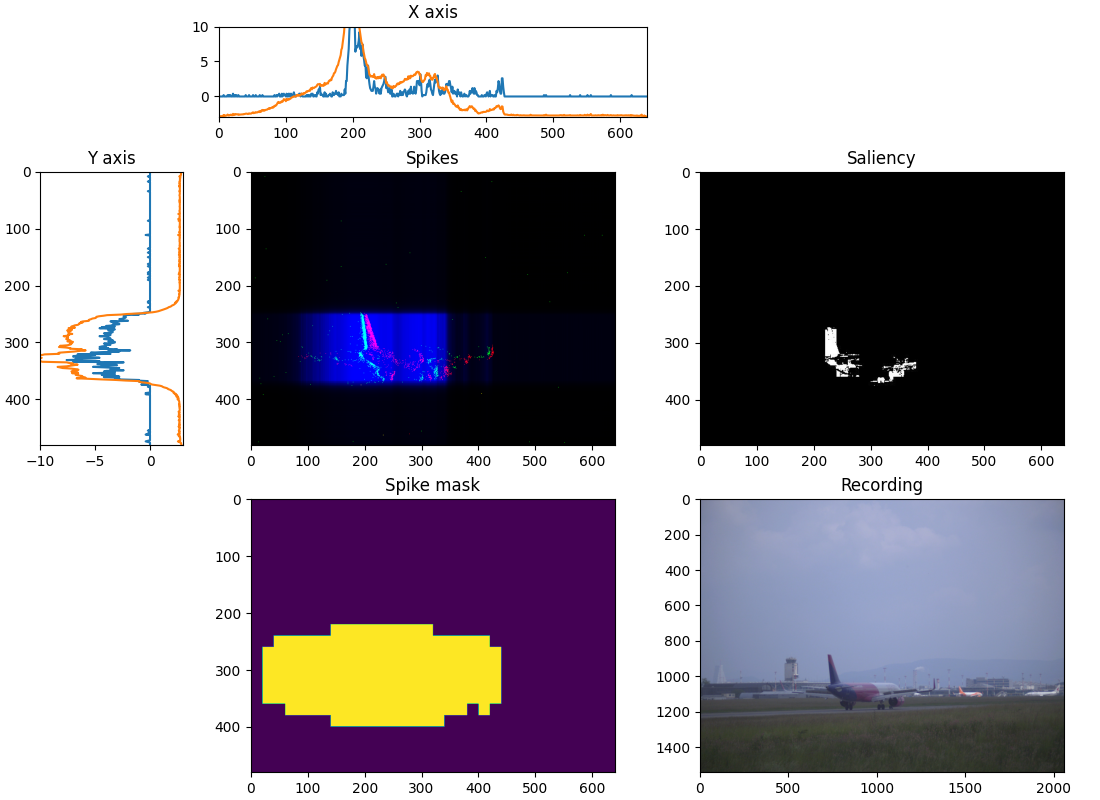
\includegraphics[width=\linewidth]{tracking/spike_opti}
		\end{subfigureth}
		\caption[Combinaison SOM et DNF par zone d'intérêt]{Un exemple de combinaison possible entre une caméra évènementielle et la détection de nouveauté avec une SOM. Les DNF travaillant sur les entrées évènementielles permettent la création d'une zone d'intérêt (image en bas à gauche). Cette zone d'intérêt sert à concentrer les efforts de la SOM là où de la nouveauté a des chances d'apparaître.}\label{fig:opti:spike}
	\end{figureth}

	Le masque est obtenu en appliquant un seuil sur la combinaison des deux DNF par le produit dyadique. La valeur du seuil a été choisie pour englober la zone d'intérêt le plus possible sans dépasser au delà. Un seuil trop bas a pour conséquence qu'une activation d'un seul DNF suffira à dépasser le seuil, et ainsi la zone d'intérêt formera une "croix" avec pour centre la vraie zone d'intérêt. Un bon seuil est donc juste assez haut pour éviter la croix, mais le plus bas possible pour ne rien perdre dans la zone d'intérêt.

	\begin{tableth}
	\caption[Gains grâce à la combinaison SOM-DNF]{Estimation de gains potentiels avec cette combinaison de SOM-DNF. Il n'y a pas beaucoup de nouveauté qui est perdue (83\% de la sortie de la SOM conservée au minimum), et les pertes sont en majorité du bruit. Les gains quand à eux peuvent aller de 2 fois plus rapide à 10 fois, en fonction de la taille du signal, et du bruit ambiant.}
	\begin{tabular}{|c|c|c|}
		\hline
		Séquence & Taux de positifs conservés & Taux d'imagettes évaluées\\
		\hline
		Plane & 98,9\% & 10\% \\
		Walk & 83,6\% & 43\% \\
		Highway & 90,8\% & 18,3\% \\
		\hline
	\end{tabular}
	\label{tab:nbr:optidnf}
	\end{tableth}

	Le tableau \ref{tab:nbr:optidnf} présente quelques métriques pour estimer les gains potentiels de cette méthode sur des séquences que nous avons enregistrées. Les gains dépendent fortement de la taille des objets en mouvements (plus ils sont gros, plus la SOM sera sollicitée), et du bruit ambiant. En effet, des mouvements sans nouveauté dans le fond d'une image solliciterons la SOM pour les classer en nouveauté ou non continuellement. Mais si il n'y a pas de signal et que les DNF ne s'activent pas à cause du bruit, la SOM peut être complètement ignorée et la caméra non évènementielle éteinte. Cela permet donc un mode d'observation passif consommant peu d'énergie (uniquement avec caméra évènementielle et DNF), qui peut automatiquement devenir actif en fonction de la scène observée.

	\newpage

	\section{Mécanisme attentionnel}

	Objectif 1 seul stimulus

	tracking de ce stimulus

	\subsection{DNF pour l'attention}

	DNF 2D en mode sélection

	Paramètres

	Besoin de nouveauté + spikes

	Figures 

	\subsection{Detection pipeline}

	Spikes -> Novelty -> Attention -> tracking -> Novelty

	\subsection{Évolutions possibles}

	Multitracking

	Advanced processing

	Memory

	\section{Conclusion}
		
\bibliographystyle{francaissc}
\bibliography{Chapitre3/Biblio}